
\section{Moduł HRT}
\subsection{Badania literaturowe}

\textbf{Zagadnienie HRT w literaturze}\\
HRT - Turbulencja Rytmu Serca - to dwufazowa odpowiedź węzła zatokowego na przedwczesny skurcz komorowy. Zjawisko turbulencji rytmu serca jest powiązane ze sprawnością odruchu z baroreceptorów,  charakteryzuje odpowiedź węzła zatokowego na przedwczesne pobudzenie komorowe (VEB lub VEP), po którym dochodzi do przyspieszenia, a następnie do zwolnienia rytmu zatokowego. Oznacza to, że czas trwania kolejnych cykli (długość odstępów RR)  początkowo jest skrócony (następuje kompensacja) i stopniowo się wydłuża. Wystąpienie turbulencji po dodatkowym skurczu komorowym jest objawem prawidłowej funkcji baroreceptorów.\\
\begin{figure}[!h]
\centerline{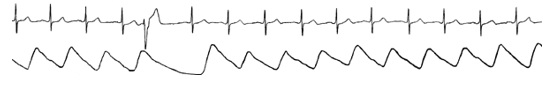
\includegraphics[scale=0.8]{HRT/rys1.jpg}}
\caption{Zapis EKG wraz z ciśnieniem krwi}
\end{figure}


HRT jest ocenione przez dwa liczbowe parametry: Turbulence Onset (początek turbulencji).  oraz Turbulence Slope (nachylenie turbulencji). Przeprowadzenie wielu badań zarówno u pacjentów bez dolegliwości sercowych jak i u ludzi chorych pozwoliło na określenie prawidłowych wartości obu parametrów.
\\Wartości prawidłowe: TO<0\%, TS>2.5ms/RR\\

\begin{figure}[!ht]
\centerline{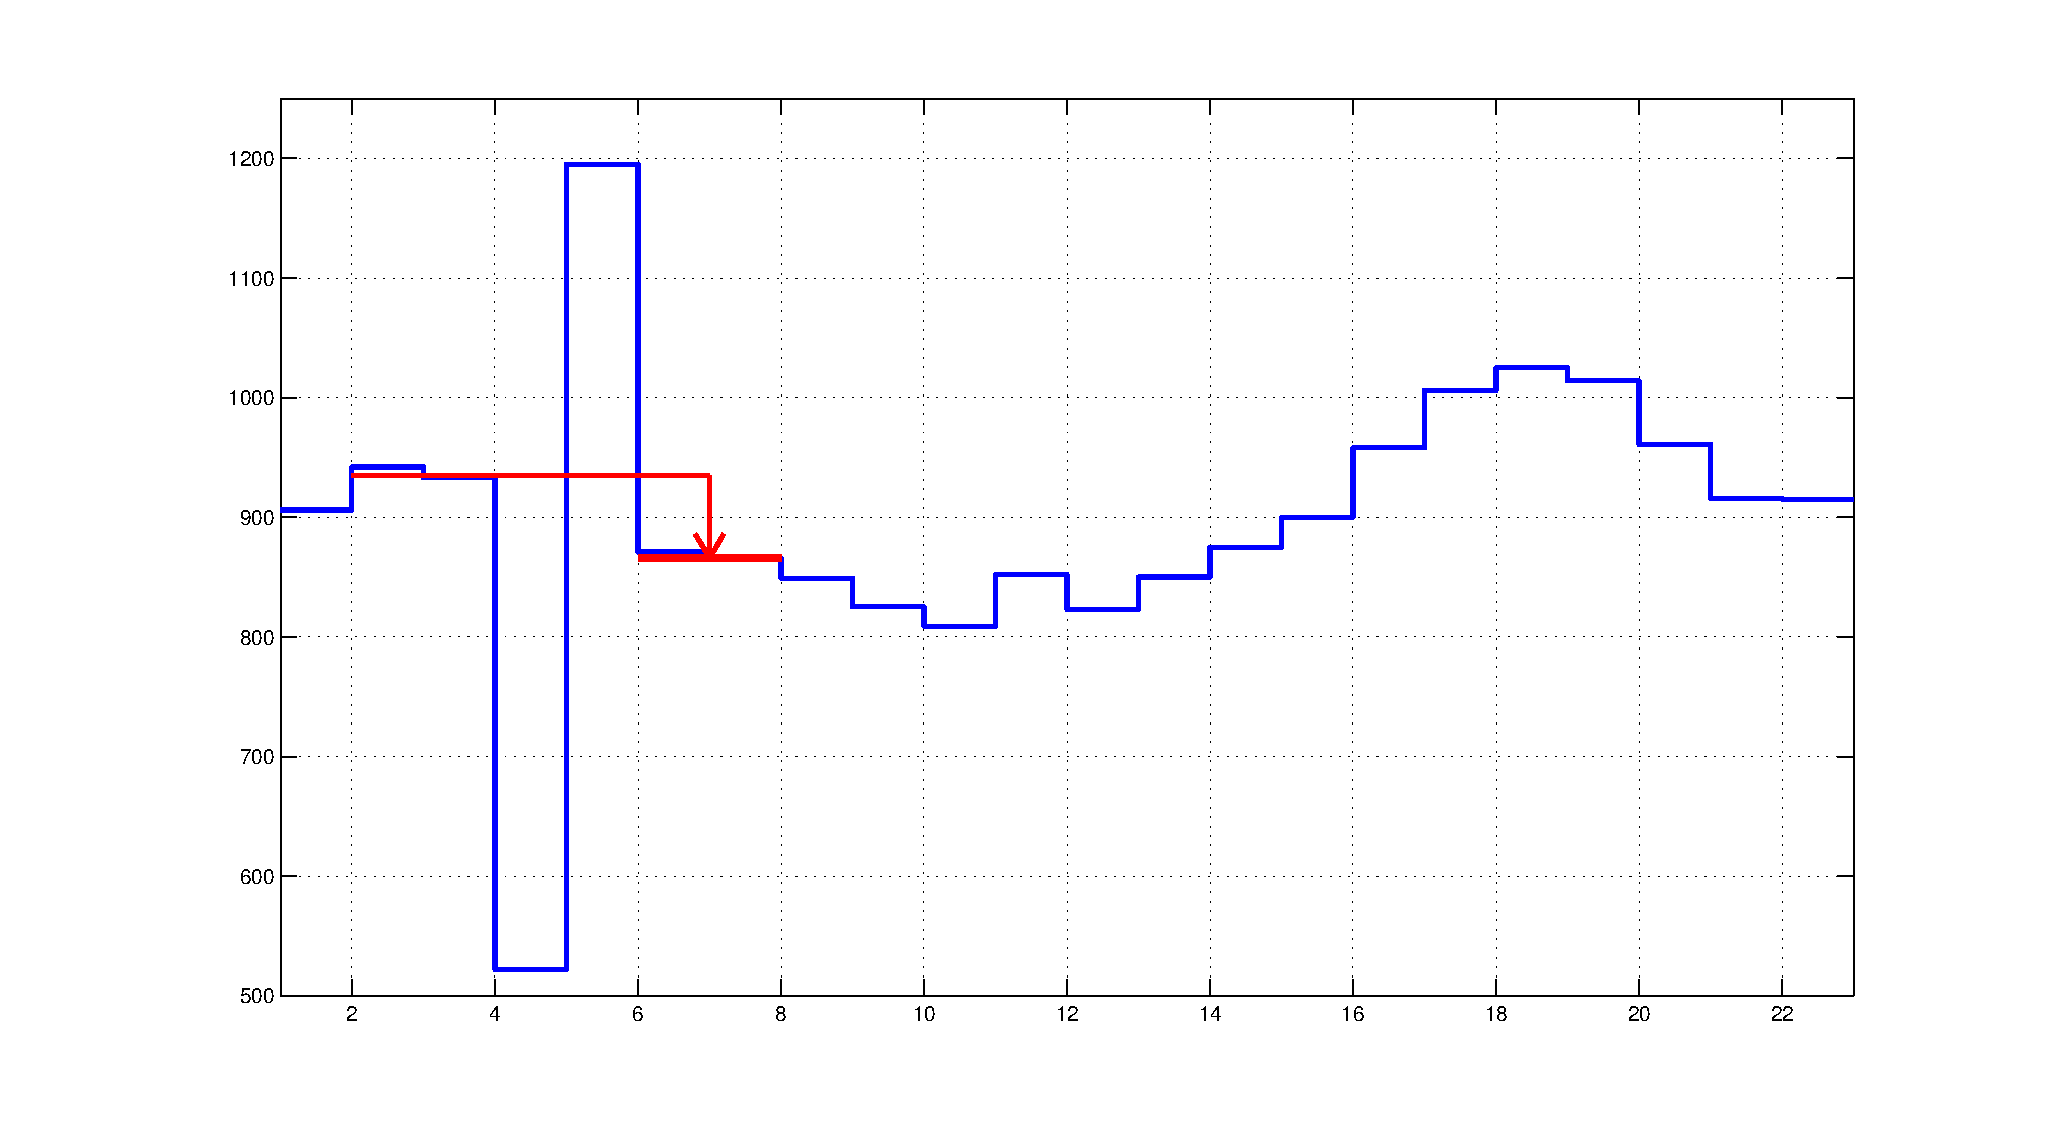
\includegraphics[scale=0.32]{HRT/HRT2.eps}}
\caption{Tachogram z graficzną reprezentacją TO}
\end{figure}

\begin{figure}[h]
\centerline{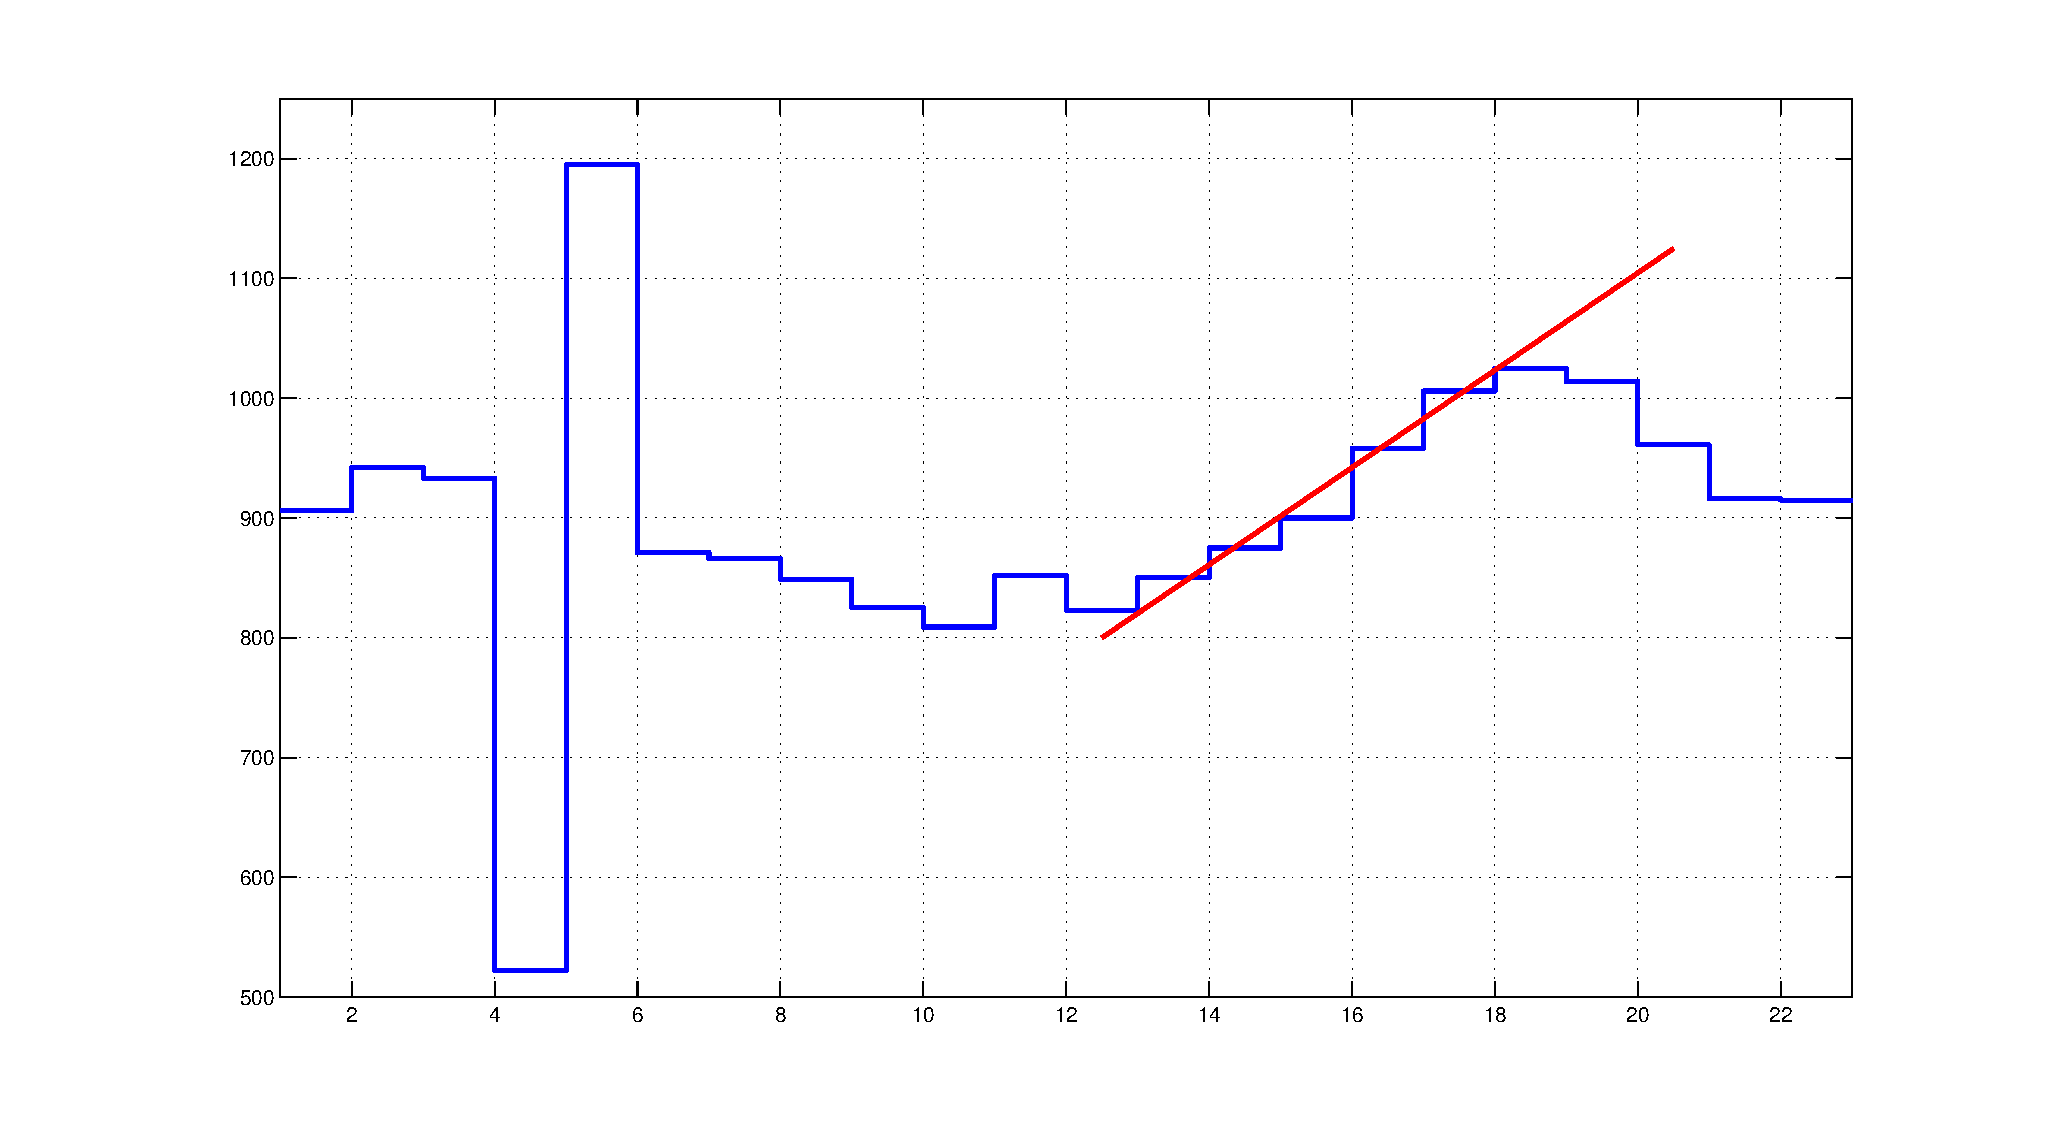
\includegraphics[scale=0.32]{HRT/HRT3.eps}}
\caption{Tachogram z graficzną reprezentacją TS}
\end{figure}

Analiza HRT okazała się przydatna w ocenie ryzyka po zawale serca. Po przeanalizowaniu danych pacjentów po zawale serca udało się ustalić, że HRT - niezależnie od innych czynników ryzyka - posiada bardzo wielką, a może nawet największą wartość predykcyjną spośród elektrokardiograficznych parametrów wykorzystywanych w celach prognostycznych. \\


\textbf{Podejście do problemu w literaturze}

\begin{itemize}
\item Wybór - filtracja danych wejściowych 
W celu uniknięcia błędów w analizie HRT przyjmuje się pewne kryteria doboru danych poddanych analizie. Bazując na odstępach czasowych interwałów RR klasyfikuje się skurcze komorowe jako przedwczesne. Skrócony RR (przedwczesny skurcz) musi być co najmniej o 20\% krótszy od wartości średniej z poprzednich 5 interwałów. Pauza po VEB ma być dłuższa co najmniej o 20\% w porównaniu do tej samej wartości średniej. Zalecana jest również filtracja ze względu na długość interwałów po i przed VEB, tak aby wykluczyć zbyt krótkie oraz zbyt długie RR’y. Przyjęto następujące kryteria dotyczące pojedynczego interwału: 
\begin{itemize}
\item RR>300ms,
\item  RR<2000,
\item RR-RR-1>200
\end{itemize}

\item Wyznaczanie parametrów z wybranych danych
Początek turbulencji oblicza się jako różnicę między średnim czasem trwania 2 pierwszych pobudzeń zatokowych następujących po VEB: (RR1 + RR2)/2, a średnim czasem trwania 2 ostatnich pobudzeń poprzedzających: (RR –1 + RR–2)/2, podzieloną przez średni czas trwania 2 ostatnich pobudzeń poprzedzających. Parametr ten jest wyrażany w procentach na podstawie wzoru, który ma postać:
\begin{equation}
TO=\frac{(RR_1+RR_2) - (RR_{-1} + RR_{-2})}{(RR_{-1} + RR_{-2})} * 100\%
\end{equation}
\end{itemize}


Nachylenie turbulencji określa się je jako największe nachylenie prostej regresji wyznaczonej z wykresu czasu trwania wybranych 5 kolejnych odstępów RR jako funkcji czasu spośród 15-20 cykli następujących po VEB. Jednostką TS jest ms/RR.

\subsection{Koncepcja proponowanego rozwiązania}
Po zapoznaniu się z literaturą przystąpiono do rozpisania schematu blokowego algorytmu (opisywany w ten sam sposób w publikacjach). 

\begin{figure}[!h]
\centerline{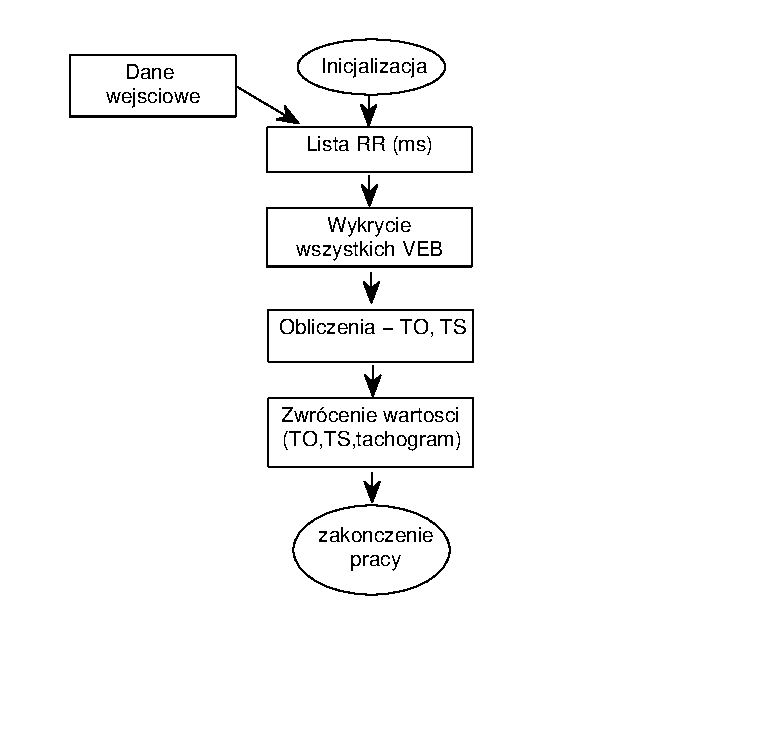
\includegraphics[scale=0.8]{HRT/HRT4.eps}}
\caption{Schemat blokowy algorytmu}
\end{figure}



\textbf{Koncepcja algorytmu}\\
Dane wejściowe:
\begin{itemize}
\item Przefiltrowany sygnał EKG, 
\item numery próbek pików R, 
\item częstotliwość próbkowania, 
\item sklasyfikowane zespoły QRS\\
\end{itemize}

Dane wyjściowe:
\begin{itemize}
\item Parametry turbulencji rytmu serca (TO, TS)
\item Dane do utworzenia wykresu pozwalającego na analizę HRT przez człowieka
\item Liczba VEB, które zostały dopuszczone do analizy \\

\end{itemize}

Kroki algorytmu:
\begin{itemize}
\item Lista RR\\
Na podstawie danych z modułu R\_PEAKS utworzenie listy z długościami kolejnych interwałów – wyrważonymi w ms (dlatego wymagana jest częstotliwość próbkowania)
\item Wykrycie VEB (przedwczesne skurcze komorowe) \\
Na podstawie danych z modułu QRS\_CLASS oraz przy użyciu wcześniej utworzonej ListyRR wybranie VEB’ów.
 Dane z modułu QRS\_CLASS muszą być dodatkowo sprawdzone, aby analiza HRT dawała poprawne wyniki.
 Warunki konieczne (przedstawione również graficznie na rysunku):\\
\begin{equation} \frac{(RR-RR_{v1})}{RR}>0.2 \end{equation}
\begin{equation} \frac{(RR_{v2} - RR)}{RR} > 0.2 \end{equation}
\begin{figure}[!ht]
\centerline{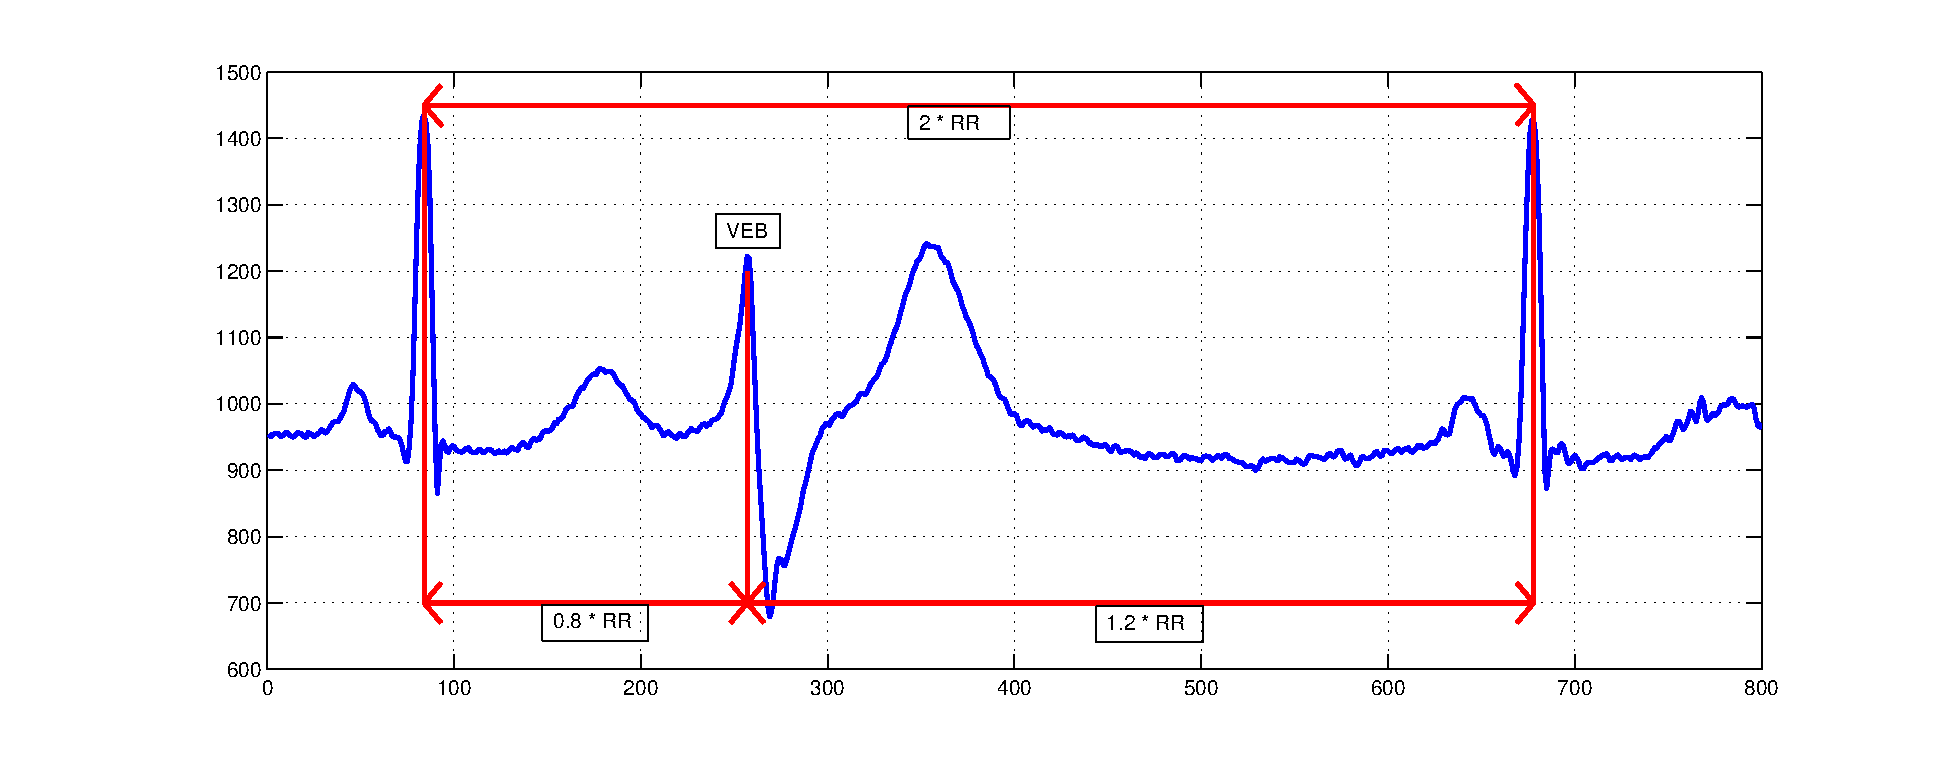
\includegraphics[scale=0.42]{HRT/HRT5.eps}}
\caption{Wykres sygnału EKG z oznaczonym VEB}
\end{figure}

\item Filtracja\\
Filtracja interwałów RR po i przed VEB, kryteria:
\begin{itemize}
\item RR>300ms,
\item RR<2000ms,
\item RR-RR\_{-1}<200ms
\end{itemize}
Filtracja interwałów RR po i przed VEB (kryteria podane w literaturze) – jeśli interwał nie spełnia warunków cały ciąg próbek odpowiadający danemu VEB nie będzie brany pod uwagę w następnym kroku algorytmu.
Wymagane jest co najmniej 5 poprawnych ciągów próbek, aby analiza była skuteczna (o nie spełnieniu danego warunku użytkownik powinien być powiadomiony) .
\item Utworzenie tachogramu dla każdego wykrytego VEB.Wymagane jest cztery próbki poprzedzające przedwczesny skurcz komorowy i dwadzieścia jeden po.
\item Obliczenia\\
\begin{itemize}
\item TO– wyliczane dla każdego VEB wg wzoru: \begin{equation} TO=\frac{(RR_1+RR_2) - (RR_{-1} + RR_{-2})}{(RR_{-1} + RR_{-2})} * 100\% \end{equation} \\Następnie wybieramy wartość średnią.
\item TS – wartość maksymalna współczynnika kierunkowego a wyliczona metodą regresji liniowej z uśrednionego tachogramu:\\
\begin{equation} a=\frac{n\sum{x_iy_i}-\sum{x_i}\sum{y_i}}{n\sum{x_i^2}-(\sum{x_i})^2}\end{equation}
\begin{equation}b=\frac{1}{n}(\sum{y_i}-a\sum{x_i})\end{equation}
\end{itemize}
\item Zwrócenie danych
\begin{itemize}
\item Liczba VEB dopuszczonych do analizy
\item TO
\item TS
\item Uśredniony tachogram
\end{itemize}
\end{itemize}


\subsection{Rezultaty i wnioski}
Przedstawiony algorytm został zaimplementowany w języku C++, oraz języku skryptowym oprogramowania Matlab. Skryptem posłużono się w celu weryfikacji i analizy działania modułu.\\ 
Działanie algorytmu było testowane na próbkach przepisanych z bazy:\\
MIT-BIH Arrhythmia Database - 106\\
Opis sygnału zawierał również informację o miejscu wystąpienia przedwczesnego skurczu komorowego (4min 23s), co było bardzo pomocne przy analizie. \\

Wycinek sygnału, w którym zaobserwowano przedwczesny skurcz został zaprezentowany graficznie 

\begin{figure}[h]
\centerline{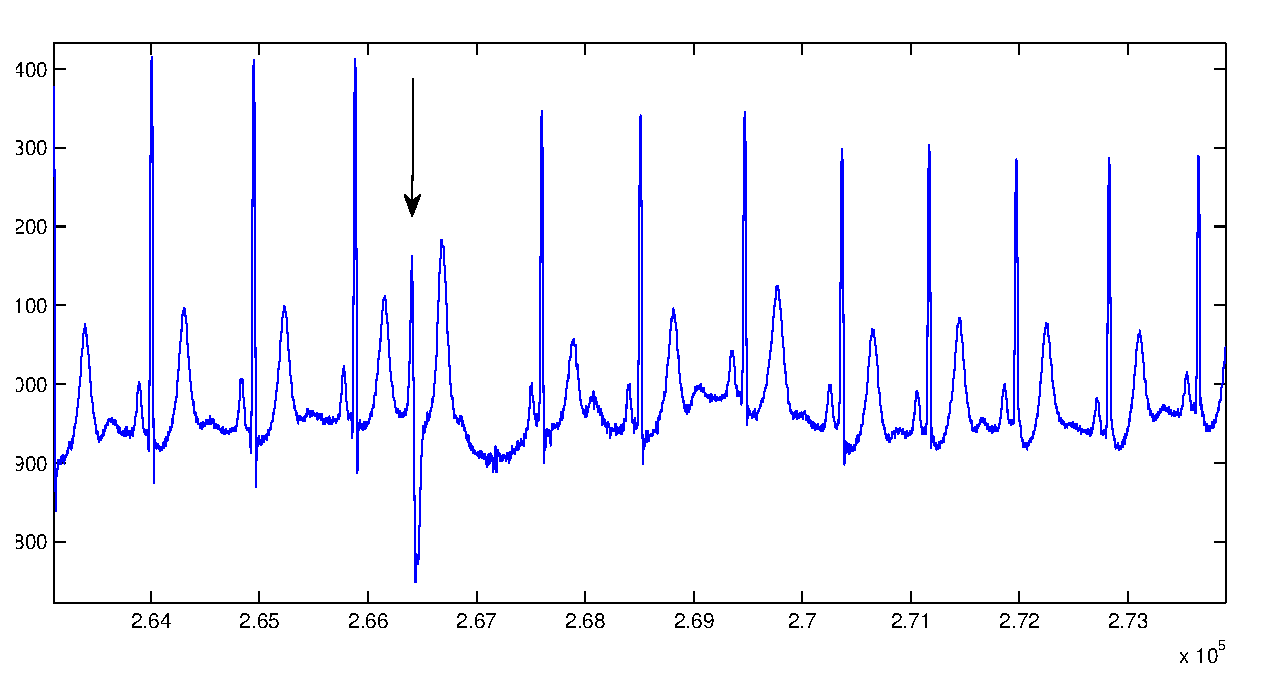
\includegraphics[scale=0.5]{HRT/HRT6.eps}}
\caption{Wykres sygnału EKG z oznaczonym VEB [mitdb/106 ~0:04:20-0:04:30]}
\end{figure}

Niestety podczas fazy testowej nie dysponowano pozostałymi modułami – R\_PEAKS, QRS\_CLASS. Przeprowadzenie testu wymagało ręcznego wprowadzenia ciągów próbek pików R (zadanie modułu R\_PEAKS). 
Zbiór testowy został dobrany w taki sposób, aby sprawdzić najważniejsze funkcje algorytmu, tj. odnajdywanie VEB spełniającego podstawowe wymagania czasowe przedstawione w poprzednim punkcie. Odstępy czasowe pików R zostały zachowane, jednak nie przepisano całego ciągu, a jedynie połączono wybrane przedziały w których odnaleziono VEB analizując sygnał EKG. Utworzony ciąg próbek pików R został przedstawiony na tachogramie.\\

\begin{figure}[!h]
\centerline{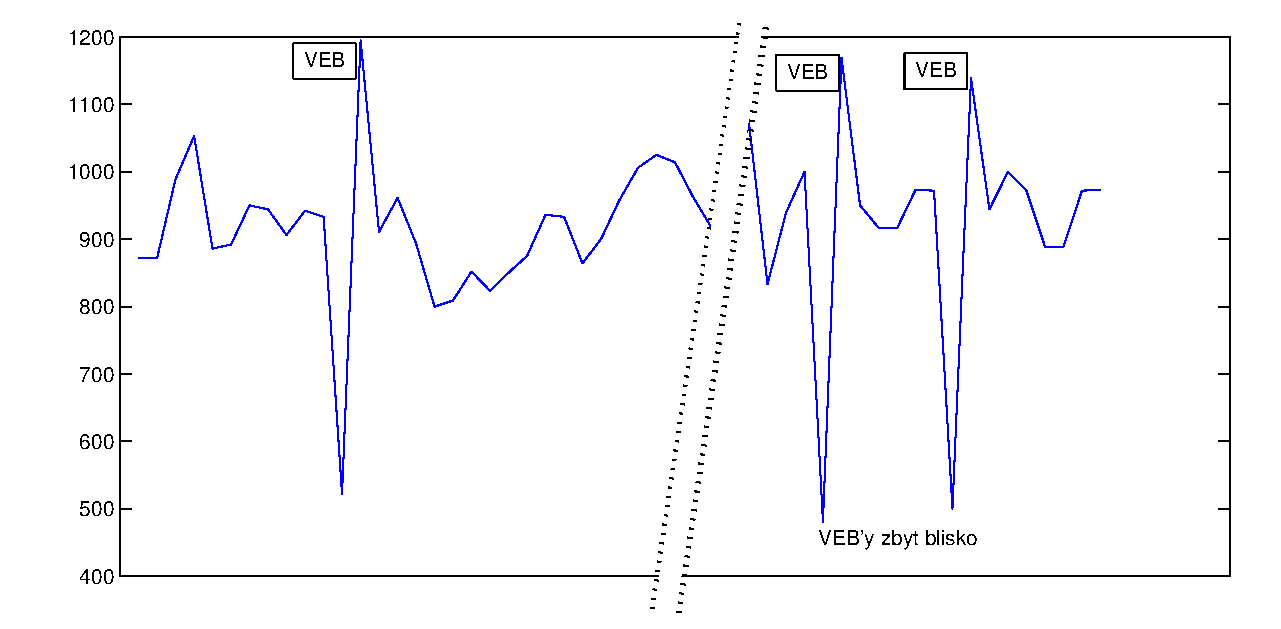
\includegraphics[scale=0.55]{HRT/HRT7.eps}}
\caption{Tachogram z oznaczonymi VEB [mitdb/106 ~(0:04:23, 0:7:25, 0:15:21)]}
\end{figure}

Na tachogramie zaznaczono kolejne skurcze, które powinny być wykryte w pierwszej fazie, ponieważ spełniają wymagania czasowe. Następnie jeśli wykryte skurcze są blisko siebie (drugi i trzeci) powinny zostać odrzucone z analizy, pierwszy VEB pozostanie. W ostatnim etapie filtracji danych sprawdzone zostaną kryteria dotyczące pojedynczych odstępów RR.\\

\begin{table}[t]
\caption{Uzyskane wyniki liczbowe}
\centerline{\begin{tabular}{|r|l| r| r|}
  \hline 
  Całkowita liczba VEB & Liczba VEB po filtracji danych & TO & TS\\
  \hline
  9 & 3 & 0.16\% & 42.8ms/RR \\
  \hline
\end{tabular}}
\end{table}
Jako uzupełnienie wyników liczbowych przedstawiono również tachogram z zaznaczoną prostą definiującą współczynnik TS:

\begin{figure}[!h]
\centerline{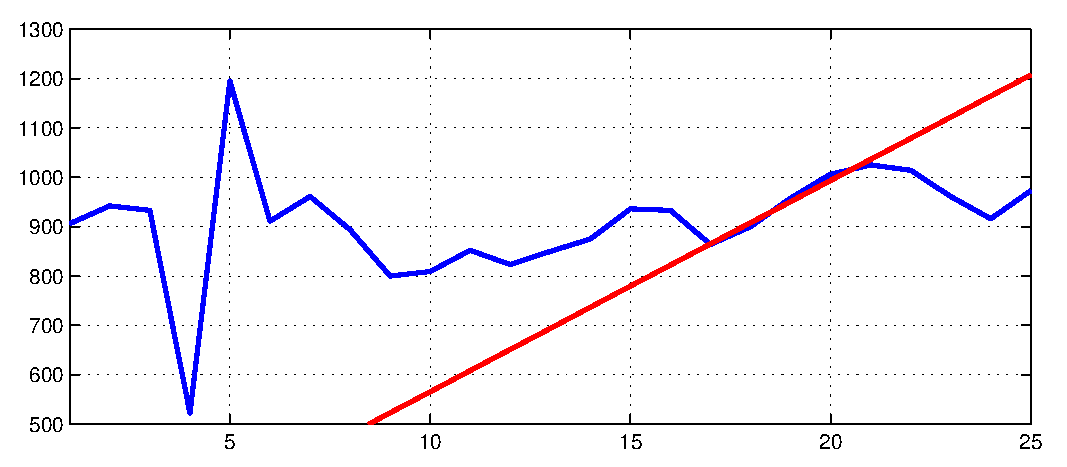
\includegraphics[scale=0.6]{HRT/HRT8.eps}}
\caption{Wyjściowy tachogram }
\end{figure}

Analiza HRT to nowa i nie do końca poznana metoda, dlatego też jedyne co można powiedzieć o otrzymanych wynikach to: współczynnik TO jest za wysoki – dla zdrowego człowieka powinien być mniejszy od 0, współczynnik TS jest odpowiedni – większy od 2.5ms/RR. Na uśrednionym tachogramie można zauważyć prawidłową pracę korekcyjną po przedwczesnym skurczu komorowym – początkowe przyspieszenie pracy serca, a następnie stopniowe spowalnianie.\\
W bazie danych nie odnaleziono danych referencyjnych do których można by było porównać otrzymane wyniki.\\
W efekcie końcowym moduł nie został połączony z QRS\_CLASS- wyszukiwanie przedwczesnych skurczy komorowych odbywa się na podstawie danych z utworzonej listy RR.


\subsubsection{Literatura}
Spis literatury związanej z modułem HRT
\begin{itemize}
\item Georg Schmidt, Raphael Schneider and Petra Barthel - Heart Rate Turbulence, Cardiac Electrophysiology Review 1999 
\item M. Zając, J. Drożdż, M. Kurpesa, E. Trzos,T. Rechciński - Turbulencja rytmu serca jako metoda oceny ryzyka nagłego zgonu sercowego
\item Heart Rate Turbulence: Standards of Measurement, Physiological Interpretation, and Clinical Use - 2008 by the American College of Cardiology Foundation
<<<<<<< HEAD
\end{itemize}
=======
\end{itemize}
>>>>>>> upstream/dev
